\documentclass[11pt]{amsart}
\usepackage{geometry} % see geometry.pdf on how to lay out the page. There's lots.
\geometry{a4paper} % or letter or a5paper or ... etc
% \geometry{landscape} % rotated page geometry

\usepackage[toc,page]{appendix}
% See the ``Article customise'' template for come common customisations

\usepackage{graphicx}	
\usepackage{listings}

\title{An Intuitive Perspective of Vendor Lead Times and Ordering Frequency}
\date{} % delete this line to display the current date

%%% BEGIN DOCUMENT
\begin{document}

\maketitle

\section{Purpose of this Note}

I'm writing this brief note to provide a simple and intuitive perspective of vendor lead time and ordering frequency. Here are some questions pertaining to Purchasing that we've been thinking about lately:

\begin{itemize}
\item Can we define a notion of ``Ideal Inventory Position'' for the most upstream nodes in our network (nodes that receive inventory from vendors)?
\item Is the current structure of lead times and order frequencies/quantities (from vendors) defective in meeting aggregate downstream demand (covering requisite guest availability for each SKU)?  
\item How do we ensure that the structure of Purchasing (lead times and order frequencies/quantities) required to meet downstream demand doesn't lead to space overflow at our most upstream nodes?
\end{itemize}

To answer the above questions, we start by stating the goal of purchasing and show some simple formulas to help develop intuition (and avoid mathematical complexity). This is not to say that our full-blown Purchasing Algorithm will compromise on mathematical rigor. We simply relax the setting here to help explain Purchasing in simple and intuitive terms.

\section{Purchasing 101}

The goal of Purchasing is to order from vendors with the appropriate speed and frequency that meets requisite downstream demand in the most cost-optimal manner. With a simple and intuitive setting, we define the notion of ``Ideal inventory Position'' at the most upstream nodes in our network, and use this notion of ``Ideal Inventory Position'' to drive the explanations and address questions pertaining to lead times and ordering frequencies. We will refer to the most upstream node in our network as $U$. Assume that node $U$ serves a large set of stores, say 50-200 stores. RDC 551 is a good example. Node $U$ will keep some safety stock (to account for downstream withdrawal uncertainty) and will also buffer some inventory due to transport-cost considerations, constrained ordering cadence, minimum order quantities, casepacks etc.
 
Let the aggregate single-epoch withdrawal from all the stores served by node $U$ be defined by a normal distribution with mean $\mu$ and standard deviation $\sigma$ (normal distribution is not a bad assumption because Central Limit Theorem is our friend here). We get nice risk-pooling benefits at node $U$, so while $\mu$ is additive over the individual stores' mean demands, $\sigma$ grows (as a function of stores) much slower than additive (eg: $\sqrt{stores}$ if correlation between stores is 0). Appendix \ref{appendix:MeanStdevFormulas} provides some mathematical detail on estimating $\mu$ and $\sigma$ from demand probabilities at the stores.
 
Let the lead time from Vendor to node $U$ be denoted by $L$ epochs, and let the ordering-cadence period for node $U$ be denoted by $R$ epochs. $L$ is quantified such that it includes lead time uncertainty (you can estimate it as mean of lead time + say 2 standard deviations of lead time uncertainty).
 
Appendix \ref{appendix:IPOHOOFormulas} derives the formulas for expected Beginning-On-Hand ($BOH_i$), Ending-On-Hand ($EOH_i$), On-Order ($OO_i$) and Inventory Position ($IP_i$ = $BOH_i + OO_i$) for each epoch $i = 0, \ldots, R - 1$ (the cycle repeats after $R$ epochs, so calculating it only for the range $i = 0, \ldots, R - 1$ suffices).

We will define the Ideal Inventory Position in epoch $i$ as $IP_i$ which is (as derived in Appendix \ref{appendix:IPOHOOFormulas}) equal to:
 
$$\mu * (L + R - i) + \Phi^{-1}(\alpha) * \sigma * \sqrt{L+R-i}$$

where $\alpha$ is the Type-1 service level provided by node $U$ to the aggregate withdrawal demand from the stores, and $\Phi$ is standard normal Gaussian Cumulative Density Function.
 
Note that $\mu$ and $\sigma$ are given to us (from guest demand forecast), and $\alpha$ can be obtained from our middle-mile Clark-Scarf algorithm for requisite guest availability (eg: if requisite guest availability is 98\%, then $\alpha$ will be roughly 99.5\% for typical assumptions of holding costs and lead times). 

Our levers are $R$ and $L$. So we will treat the Ideal Inventory Position as a function of $L$ and $R$, denoted as $IIP_i(L, R)$.

$$IIP_i(L, R) = \mu * (L + R - i) + \Phi^{-1}(\alpha) * \sigma * \sqrt{L+R-i}$$

How do we interpret the above formula? This formula says that for any choice of $L$ and $R$, you can meet the downstream aggregate withdrawal (to meet requisite guest availability) by maintaining an average inventory position of $IIP_i(L,R)$ at node $U$ in epoch $i$ of the $R$-epochs-cycle. And you can maintain the average inventory position of $IIP_i(L,R)$ by structuring a vendor lead time of $L$, an ordering-cadence period of $R$, and an average order quantity of $\mu * R$. But note that high values of $L$ or $R$ will yield high values of $IIP_i(L,R)$. So our job should be to keep $L$ and $R$ as low as possible. So let us understand the factors influencing $L$ and $R$ so we know how low we can get on $L$ and $R$.

\section{Factors influencing $L$}
Note that vendor lead time is the time from placing an order to physically receiving the requested inventory. So it includes the transportation time plus the processing time. The factors affecting $L$ are:
\begin{itemize}
\item Distance from the vendor creates a basic lower bound on $L$
\item Vendor time/process-constraints creates a lower bound on the processing time and hence, a lower bound on $L$
\item Requiring low and reliable lead time could involve writing a vendor contract that might be expensive to us (since it involves precision and robustness from the vendor).
\end{itemize}

\section{Factors influencing R}
\begin{itemize}
\item Constraints on shipment days and delivery days would constrain $R$.
\item Vendor Casepack (VCP) creates a constraint on $R$. $R$ can be approximated as $\lfloor \frac {VCP} {\mu} \rfloor$.
\item Minimum Order Quantities will also create a constraint on $R$.
\item Transport costs might prevent $R$ from getting too small (indeed, our Purchasing algorithm essentially solves for the optimal $R$, balancing transport costs against the inventory costs at node $U$).
\item On the flip side, space constraints at node $U$ will force $R$ to be small enough because large $R$ can lead to overflow of inventory at node $U$.
\end{itemize}

\section{Insights and Analysis associated with Purchasing}

The simple formula for Ideal Inventory Position serves as an excellent base for performing quick analyses and deriving valuable insights into various questions we would ask pertaining to purchasing. Let us look at two such questions to illustrate the point.

\begin{enumerate}

\item {\bf Is the current structure of lead times and order frequencies/quantities at node $U$ defective in meeting aggregate downstream demand (covering requisite guest availability for each SKU)?} Here's how we can tackle this problem: Set up an equation that equates the formula for Ideal Inventory Position in epoch $i$ ($ = \mu * (L + R - i) + \Phi^{-1}(\alpha) * \sigma * \sqrt{L+R-i}$) to the observed Inventory Position at node $U$ in epoch $i$. In this equation, set the parameters $L$ and $R$ to the lead times and ordering cadence-periods observed in recent data on vendor ordering. Set the parameters $\mu$ and $\sigma$ based on the calculation in Appendix \ref{appendix:MeanStdevFormulas}. Now, solve for the free parameter $\alpha$. Let us denote the solved-for value of $\alpha$ as $\hat{\alpha}$ (we call this the ``Implied service level provided by node $U$ to the aggregate withdrawal demand from the stores'', shortened to simply "Implied Service Level"). If the Implied Service Level $\hat{\alpha}$ turns out to be lower than the appropriate service level to meet requisite guest availability (the translation from guest availability to node $U$'s service level is directly obtained from Clark-Scarf), then the current structure of lead times and order frequencies/quantities are defective in meeting aggregate downstream demand. Moreover, we are able to quantify the degree of the defect.

\item {\bf How do we ensure that the structure of Purchasing (lead times and order frequencies/quantities) required to meet downstream demand doesn't lead to space overflow at our most upstream nodes?} We consider the maximum Expected Beginning-on-Hand Inventory at node $U$ across the $R$-epochs-cycle. As established in Appendix \ref{appendix:IPOHOOFormulas}, $Max EBOH =  \mu * R + \Phi^{-1}(\alpha) * \sigma * \sqrt{L+R}$. Based on the structure of lead times and order frequencies, we know $L$ and $R$. We derive $\alpha$ from the requisite guest availability, and we get $\mu$ and $\sigma$ from the formulas in Appendix \ref{appendix:MeanStdevFormulas}. Now simply plug in $L, R, \alpha, \mu, \sigma$ in the above formula for $ Max EBOH$, and convert the units to cubic volume. Then sum up this calculated cubic volume across all the SKUs served by node $U$. If this aggregate cubic volume is within the space available at node $U$, then we know that the structure of Purchasing required to meet downstream demand will not lead to space overflow at node $U$.

\end{enumerate}

\begin{appendices}

\section{Mean and Standard Deviation of Withdrawal from the Most Upstream Node}
\label{appendix:MeanStdevFormulas}

This appendix provides simple formulas to estimate $\mu$ and $\sigma$ (the mean and standard deviation of single-epoch withdrawal from the most upstream node). 

$$\mu = \sum_{i=1}^n \mu_i$$

where $\mu_i$ refers to the single-epoch mean demand at store $i$, for all $i = 1, \ldots, n$

$$\sigma = \sqrt{\sum_{i=1}^n \sum_{j=1}^n \sigma_i \sigma_j \rho_{i,j} }$$

where $\sigma_i$ refers to the standard deviation of single-epoch demand at store $i$ and $\rho_{i,j}$ refers to the correlation of single-epoch demand between stores $i$ and $j$, for all $i, j = 1, \ldots, n$.

If we assume all the stores have the same single-epoch mean demand $\mu_s$ and the same standard deviation of single-epoch demand $\sigma_s$ and each pair of stores has the same correlation $\rho$ for single-epoch demand, then the above formulas simplify to:

$$\mu = \mu_s * n$$

$$\sigma = \sqrt{ n * \sigma_s^2 + n * (n-1) * \sigma_s^2 * \rho} = \sigma_s \sqrt{n} \sqrt{1 + (n-1) \rho}$$

and if $\rho = 0$, then the formula further simplifies to:

$$\sigma = \sigma_s * \sqrt{n}$$

\section{Formulas for Inventory Position, On-Hand and On-Order}
\label{appendix:IPOHOOFormulas}

Let the aggregate single-epoch withdrawal from all the stores served by node $U$ be defined by a normal distribution with mean $\mu$ and standard deviation $\sigma$ (normal distribution is not a bad assumption because Central Limit Theorem is our friend here). Denote the lead time from Vendor to node $U$ by $L$ epochs and the ordering-cadence period for node $U$ by $R$ epochs. $L$ is quantified such that it includes lead time uncertainty (you can estimate it as mean of lead time + say 2 standard deviations of lead time uncertainty). Assume $\alpha$ is the Type-1 service level provided by node $U$ to the aggregate withdrawal demand from the stores. We shall assume that we place orders and receive shipments at the beginning of epochs.

We are interested in establishing formulas for the following quantities for each epoch $i = 0, \ldots, R - 1$ (the cycle repeats after $R$ epochs, so calculating it only for the range $i = 0, \ldots, R - 1$ suffices):

\begin{itemize}
\item Ideal Inventory Position ($IIP_i$)
\item Expected Beginning-On-Hand ($EBOH_i$)
\item Expected Ending-On-Hand ($EEOH_i$)
\item Expected On-Order ($EOO_i$)
\item Expected Inventory Position ($EIP_i = EBOH_i + EOO_i$)
\end{itemize}

Since we order once every $R$ epochs and since mean withdrawal per epoch is $\mu$, we can assume without loss of generality that in epoch 0, the expected order quantity is $\mu * R$ and this order will arrive from the vendor after $L$ epochs (if $L > R$, the shipment received in epoch $L \bmod R$ was ordered in an earlier $R$-epochs-cycle). 

Let us first figure out what is the ideal inventory position ($IIP_i$) when you are at epoch $i$ for all $i = 0, \ldots, R - 1$. The inventory position needs to be adequate enough in epoch $i$ such that the on-hand inventory at the end of epoch $R + L - 1$ is greater than or equal to 0 with probability $\alpha$ (i.e., just before the first receipt of inventory that is not included in the On-Order in epoch $i$. This receipt happens at the beginning of epoch $R+L$). In other words, $IIP_i = F_{L+R-i}^{-1}(\alpha)$ where $F_{L+R-i}$ is the cumulative probability distribution function of the aggregate demand in the next $L+R-i$ epochs starting at epoch $i$. Assuming identical and independent gaussian $N(\mu, \sigma^2)$ demand in each epoch, this formula for $IIP_i$ reduces to:

$$IIP_i = \mu * (L + R - i) + \Phi^{-1}(\alpha) * \sigma * \sqrt{L+R - i}$$

where $\Phi$ is standard normal Gaussian Cumulative Density Function.

Ideal Inventory Position $IIP_i$ ensures that we maintain a Type-1 availability of $\alpha$. Expected Inventory Position $EIP_i$ will be a bit different than $IIP_i$, although $IIP_0 = EIP_0$ (this means we expect the inventory position to be equal to the ideal inventory position at the beginning of epoch 0, i.e., when an order is placed). Now as the epochs roll in ($ i = 1, \ldots, R - 1$), $EIP_i = EIP_0 - \mu * i = IIP_0 - \mu * i$ (because the expected withdrawal in each epoch is $\mu$). So,

$$EIP_i = \mu * (L + R - i) + \Phi^{-1}(\alpha) * \sigma * \sqrt{L+R}$$

Note that in epochs $0, \ldots, (L-1) \bmod R$, we have $\lceil \frac L R \rceil$ shipments in-transit (each with an expected quantity of $\mu * R$). Hence,

For all $i = 0, \ldots, (L - 1) \bmod R$,
$$ EOO_i = \lceil \frac L R \rceil * \mu * R $$
For all $i = ((L - 1) \bmod R) + 1, \ldots, R - 1$,
$$ EOO_i = \lfloor\frac L R \rfloor * \mu * R $$

For all $i = 0, \ldots, (L - 1) \bmod R$, 
$$ EBOH_i = EIP_i - EOO_i = \mu * (L  - i + R * (1 - \lceil \frac L R \rceil)) + \Phi^{-1}(\alpha) * \sigma * \sqrt{L+R} $$
For all  $i = ((L - 1) \bmod R) + 1, \ldots, R - 1,$
$$ EBOH_i = EIP_i - EOO_i = \mu * (L - i + R * (1 - \lfloor \frac L R \rfloor)) + \Phi^{-1}(\alpha) * \sigma * \sqrt{L+R} $$

For all $i = 0, \ldots, (L - 1) \bmod R$,
$$ EEOH_i = EBOH_i - \mu = \mu * (L - (i + 1) + R * (1 - \lceil \frac L R \rceil)) + \Phi^{-1}(\alpha) * \sigma * \sqrt{L+R} $$
For all $i = ((L - 1) \bmod R) + 1, \ldots, R - 1$,
$$ EEOH_i =  EBOH_i - \mu = \mu * (L  - (i + 1) + R * (1 - \lfloor \frac L R \rfloor)) + \Phi^{-1}(\alpha) * \sigma * \sqrt{L+R}$$

Here's an example graphical illustration of the sawtooth for $IIP$, $EIP$ and $EBOH$ (To experiment with different values of $L, R, \mu, \sigma, \alpha$ and plot the sawtooth in the above graphical format, use the Python code in Appendix \ref{appendix:PythonCode}:

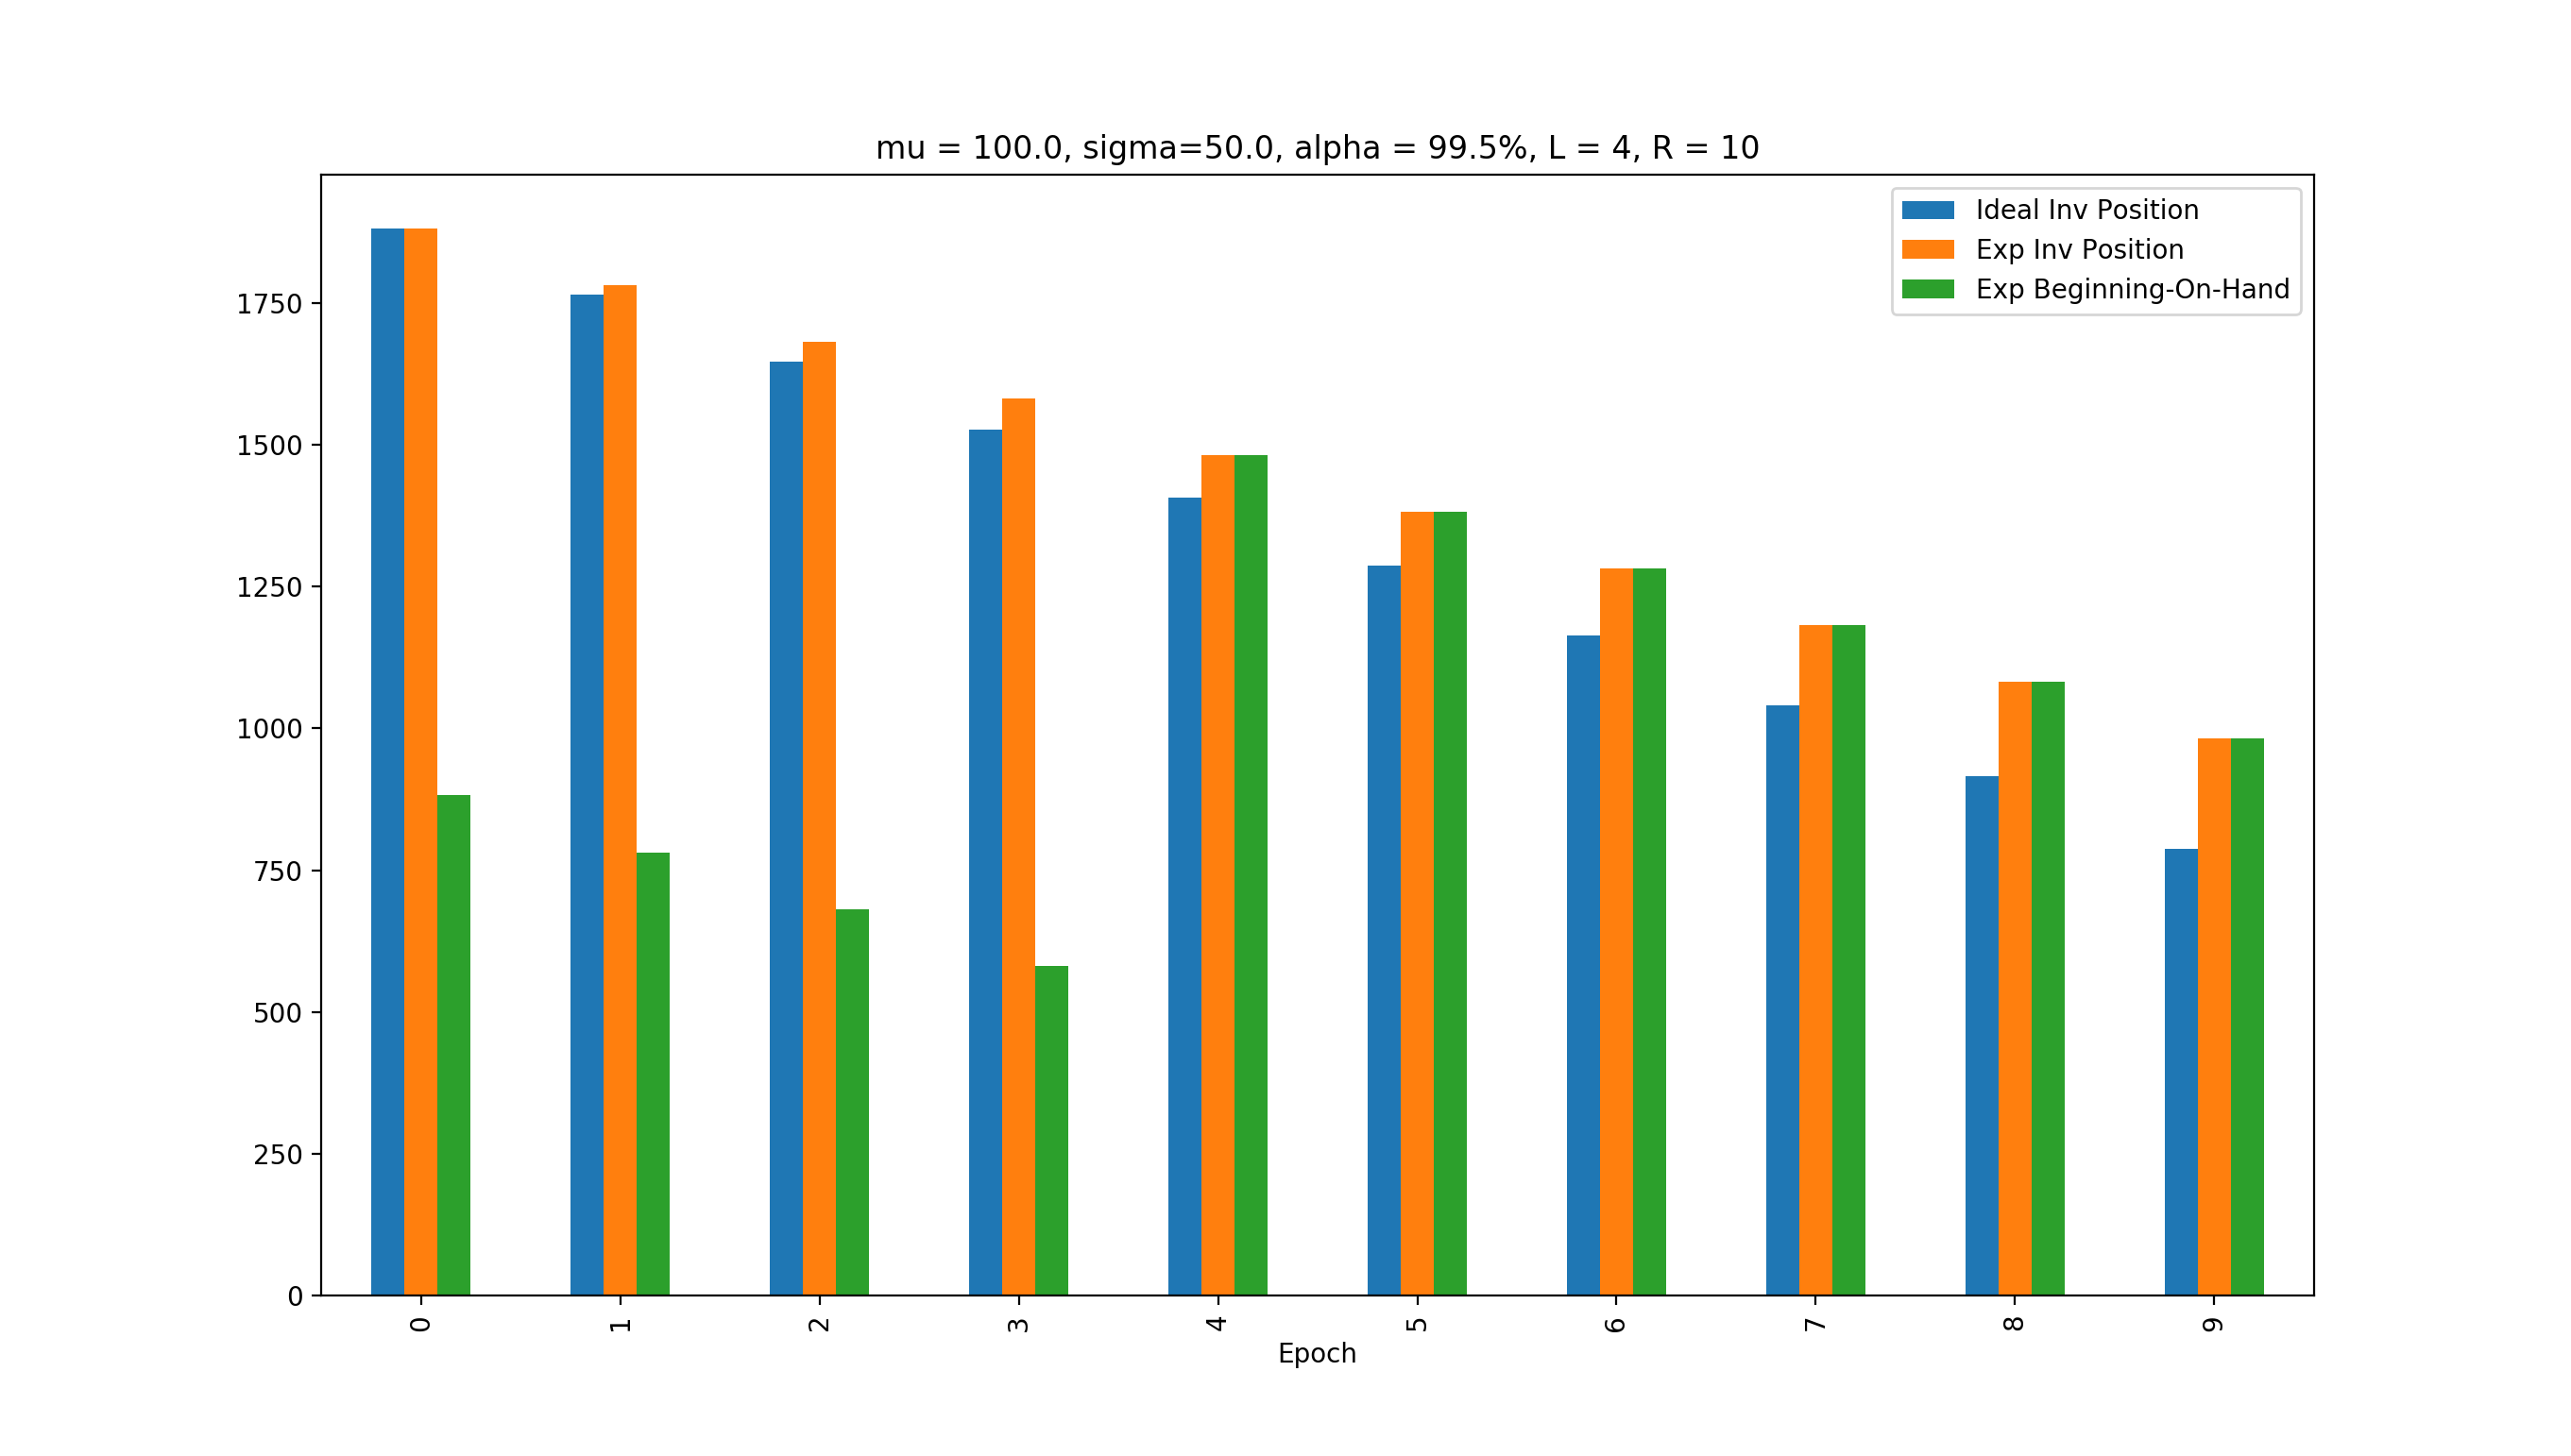
\includegraphics[height=80mm, width=130mm]{Purchasing.png}



Expected Inventory Position is maximum in epoch $0$ (when the order is placed). Hence,

$$Max EIP = EIP_0 = IIP_0 = \mu * (L + R) + \Phi^{-1}(\alpha) * \sigma * \sqrt{L+R}$$

Average Expected Inventory Position across the cycle of epochs $0, \ldots, R - 1$

$$\overline{EIP} = \mu * (L + \frac {R + 1} 2) + \Phi^{-1}(\alpha) * \sigma * \sqrt{L+R}$$

Average Expected On-Order across the cycle of epochs $0, \ldots, R - 1$

$$\overline{EOO} = \mu * L$$

Expected Beginning-On-Hand is maximum in epoch $L \bmod R$ (when a shipment is received). Hence,

$$Max EBOH = EBOH_{L \bmod R} = \mu * R + \Phi^{-1}(\alpha) * \sigma * \sqrt{L+R}$$

Average Expected Beginning-On-Hand across the cycle of epochs $0, \ldots, R - 1$

$$\overline{EBOH} = \overline{EIP} - \overline{EOO} = \mu * \frac {R + 1} 2 + \Phi^{-1}(\alpha) * \sigma * \sqrt{L+R} $$

Expected Ending-On-Hand is minimum in epoch $(L - 1) \bmod R$ (just before a shipment is received). Hence,

$$Min EEOH = EEOH_{(L - 1) \bmod R} = \Phi^{-1}(\alpha) * \sigma * \sqrt{L+R}$$

Average Expected Ending-On-Hand across the cycle of epochs $0, \ldots, R - 1$

$$\overline{EEOH} = \overline{EBOH} - \mu = \mu * \frac {R - 1} 2 + \Phi^{-1}(\alpha) * \sigma * \sqrt{L+R}$$

\section{Python Code for the above formulas and Sawtooth Plotting}
\label{appendix:PythonCode}

\begin{lstlisting}[language=Python]
from scipy.stats import norm
from math import sqrt, ceil
import pandas as pd
import matplotlib.pyplot as plt


def get_sawtooth(mu, sigma, alpha, L, R):
    iip = [mu * (L + R - i) + norm.ppf(alpha) * sigma * sqrt(L + R - i)
           for i in range(R)]
    eip = [mu * (L + R - i) + norm.ppf(alpha) * sigma * sqrt(L + R)
           for i in range(R)]
    eoo = [mu * R * (int(ceil(float(L) / R)) - (1 if i > (L - 1) % R else 0))
           for i in range(R)]
    eboh, eeoh = zip(*[(i - o, i - o - mu) for o, i in zip(eoo, eip)])
    sawtooth = pd.DataFrame({
        "Ideal Inv Position": iip,
        "Exp Inv Position": eip,
        "Exp Beginning-On-Hand": eboh,
        "Exp Ending-On-Hand": eeoh,
        "Exp On-Order": eoo
    })
    sawtooth.index.name = "Epoch"
    return sawtooth


if __name__ == "__main__":
    mu = 100.0
    sigma = 50.0
    alpha = 0.995
    L = 4
    R = 10
    sawtooth = get_sawtooth(mu, sigma, alpha, L, R)
    title = "mu = %.1f, sigma=%.1f, alpha = %.1f%%, L = %d, R = %d" % \
        (mu, sigma, alpha * 100, L, R)
    sawtooth.plot(
        y=[
           "Ideal Inv Position",
           "Exp Inv Position",
           "Exp Beginning-On-Hand"
        ],
        kind="bar",
        title=title
    )
    plt.show()
    
\end{lstlisting}

\end{appendices}

\end{document}